\section{Basics of Reinforcement Learning}
\label{sec:reinforcement_learning}

\begin{frame}{The Reinforcement Learning Framework}
\begin{figure}[t]
	\centering
	\begin{tikzpicture}[node distance = 6em, auto, thick]
		\onslide<2->{%
			\node at (4, 0) (Environment) {\includegraphics[width=3cm]{Images/environment}};
			\node at (4, 2) {\LARGE Environment};
			\node at (4, -2) {\LARGE $\calP$, $\calR$};
		}
		
		\onslide<3->{%
			\node at (-4, 0) (Agent) {\includegraphics[width=3cm]{Images/agent}};
			\node at (-4, 2) {\LARGE Agent};
			\node at (-4, -2) {\LARGE $\pi$};
		}
		
		\onslide<4->{%
		\draw [->, line width=5pt, Blue] (Environment) to [bend right=35] (Agent);
		\node at (0, 2.5) {\Large State $S_t$};
		}
		
		\onslide<5|handout:0>{%
		\node[draw=SteelBlue, circle, line width=3pt, minimum size=1cm] at (-4, -2) {};
		}
		
		\onslide<6->{%
		\draw [->, line width=5pt, SteelBlue] (Agent) to [bend right=35] (Environment);
		\node at (0, -2.5) {\Large Action $A_t$};
		}
		
		\onslide<7|handout:0>{%
		\node[draw=SteelBlue, circle, line width=3pt, minimum size=1cm] at (3.56, -2) {};	
		}
		
		\onslide<8|handout:0>{%
		\node[draw=SteelBlue, circle, line width=3pt, minimum size=1cm] at (4.42, -2) {};	
		}
					
		\onslide<9->{%
		\draw [->, line width=5pt, LightSteelBlue] (Environment) to (Agent);
		\node at (0, 0.5) {\Large Reward $R_{t+1}$};
		}		
	\end{tikzpicture}
\end{figure}
\end{frame}

\begin{frame}{Mathematical Formulation}
	\onslide<1->{%
	\textbf{State-value function}
		\begin{equation*}
			V_\pi(s) = \E[\pi]{\sum_{t=0}^{\infty} \gamma^t R_{t+1} \Big| S_0 = s}
		\end{equation*}
	}
	
	\onslide<2->{%
	\textbf{Action-value function}
		\begin{equation*}
			Q_\pi(s, a) = \E[\pi]{\sum_{t=0}^{\infty} \gamma^t R_{t+1} \Big| S_0 = s, A_0 = a}
		\end{equation*}
	}
	
	\onslide<3->{
	\textbf{Optimal value functions}
		\begin{equation*}
			V_*(s) = \max_\pi V_\pi(s) \;\;\;\;\; Q_*(s, a) = \max_\pi Q_\pi(s, a)
		\end{equation*}
	}
	
	\onslide<4->{
	\textbf{Optimal policy}
		\begin{equation*}
			\pi_* \;\text{s.t.}\; V_{\pi_*} (s) = V_*(s),\; \forall s \in \S
		\end{equation*}
	}
\end{frame}

\begin{frame}{Taxonomy of RL Algorithms}
\begin{figure}[t]
	\centering
	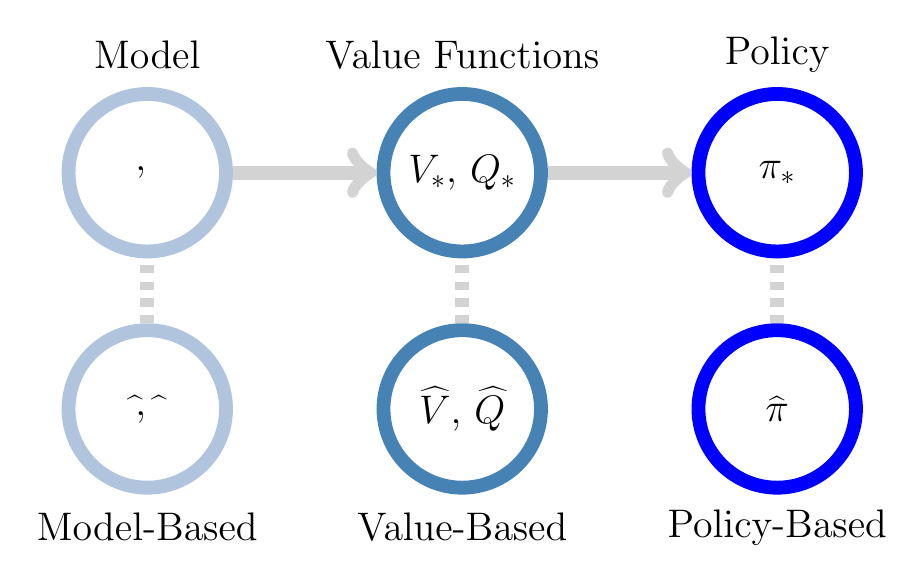
\begin{tikzpicture}[node distance = 6em, auto, thick]
		
		\onslide<1->{%
			\node [draw=LightSteelBlue, circle, line width=5pt, minimum size=2cm] at (-4, 0) (Model) {\Large $\calP$, $\calR$};
			\node at (-4, 1.5) {\Large Model};
		}
		
		\onslide<2->{%
			\node [draw=SteelBlue, circle, line width=5pt, minimum size=2cm] at (-0, 0) (Value) {\Large $V_*$, $Q_*$};
			\node at (0, 1.5) {\Large Value Functions};
			\draw [->, line width=5pt, LightGray] (Model) to (Value);
		}

		\onslide<3->{%
			\node [draw=Blue, circle, line width=5pt, minimum size=2cm] at (4, 0) (Policy) {\Large $\pi_*$};
			\node at (4, 1.5) {\Large Policy};
			\draw [->, line width=5pt, LightGray] (Value) to (Policy);
		}
		
		\onslide<4->{%
			\node [draw=LightSteelBlue, circle, line width=5pt, minimum size=2cm] at (-4, -3) (ApproxModel) {\Large $\widehat{\calP}$, $\widehat{\calR}$};
			\node at (-4, -4.5) {\Large Model-Based};
			\draw [dashed, line width=5pt, LightGray] (ApproxModel) to (Model);
		}
		
		\onslide<5->{%
			\node [draw=SteelBlue, circle, line width=5pt, minimum size=2cm] at (0, -3) (ApproxValue) {\Large $\widehat{V}$, $\widehat{Q}$};
			\node at (0, -4.5) {\Large Value-Based};
			\draw [dashed, line width=5pt, LightGray] (ApproxValue) to (Value);
		}
		
		\onslide<6->{%
			\node [draw=Blue, circle, line width=5pt, minimum size=2cm] at (4, -3) (ApproxPolicy) {\Large $\widehat{\pi}$};
			\node at (4, -4.5) {\Large Policy-Based};
			\draw [dashed, line width=5pt, LightGray] (ApproxPolicy) to (Policy);
		}
	\end{tikzpicture}
\end{figure}
\end{frame}




